\documentclass[11pt]{article}

\usepackage{listings} % Paquete para insertar códigos desde fichero

\usepackage[usenames,dvipsnames]{color} % Paquete para establecer colores por el nombre
\usepackage{mdframed} % Paquete para los recuadros de los códigos
\usepackage[utf8]{inputenc} % Para poner acentos y eñes directamente.
\usepackage{anysize} % Para establecer el margen
\usepackage{graphicx}
\usepackage{hyperref}
\usepackage[nottoc]{tocbibind}
\usepackage{framed, color}



\title{\textbf{Aplicaciones Micro-Robóticas\\
		       Proyecto de visión por computador con OpenCV}}
\author{\\Iván Félix Álvarez García\\\\\\
		\includegraphics[scale=0.45]{logo_uca}\\
		Universidad de Cádiz}
\date{30 de mayo de 2014}


\definecolor{gray}{rgb}{0.4,0.4,0.4}
\definecolor{darkblue}{rgb}{0.0,0.0,0.6}
\definecolor{cyan}{rgb}{0.0,0.6,0.6}

\lstset{
  basicstyle=\ttfamily,
  columns=fullflexible,
  showstringspaces=false,
  commentstyle=\color{gray}\upshape
}

\lstdefinelanguage{XML}
{
  morestring=[b]",
  morestring=[s]{>}{<},
  morecomment=[s]{<?}{?>},
  stringstyle=\color{black},
  identifierstyle=\color{darkblue},
  keywordstyle=\color{cyan},
  morekeywords={xmlns,version,type}% list your attributes here
}


\marginsize{2cm}{2cm}{1cm}{3cm} % Establecemos los margenes
		
\begin{document}
\maketitle
\newpage

\section{Introducción}

Este documento tiene como objetivo explicar el algoritmo de forma visual, sin entrar en detalle de implementación para que, junto a las tomas de decisión que se han tenido que tomar, mostrar la trayectoria que he seguido a lo largo del proyecto.
\\
Los pasos que voy a explicar son los que hay que tener en cuenta en todo proyecto orientado a la percepción artificial:

\begin{enumerate}
\item Captación.
\item Preproceso.
\item Segmentación.
\item Reconocimiento.
\item Actuación.
\end{enumerate}

\section{Captación de la información}
En esta etapa se tiene en mente emplear una cámara para que el robot sea capaz de ver su zona de trabajo y localizar así los distintos cuadrados de colores.

\begin{center}\includegraphics[scale=0.05]{img1}\end{center}

\noindent En un principio se tenía en mente que la cámara estuviese tomando frames constantemente pero, en la última semana, hemos observado que podemos tomar capturas en momentos determinados, consiguiendo con ello, un coste computacional menor al no tener que estar periódicamente realizando cálculos sobre todos los frames capturados.

\section{Preprocesado de los frames}
La imagen que recibimos de la cámara tiene un tamaño relativamente grande. Al comienzo del desarrollo del algoritmo, se estaba empleando la cámara de un teléfono móvil que generaba imágenes con una resolución de \textit{3264x1952} píxeles, por lo que generaba diversos problemas derivados de su tamaño, como son: la cantidad de píxeles que se deben de manejar y el ruido (como son las sombras u otros defectos provocados por el ambiente) que se ve aumentado también por la cantidad de píxeles que se tienen.
\\
Para ello, opté por reducir la imagen a una tercio de su tamaño. Esto tiene algo bueno y algo malo. Por una parte, el ruido \textit{puede} llegar a ser despreciable, pero por otra, estamos perdiendo información. ¿Esto es un problema? En nuestro caso no, ya que, aunque perdamos ciertos píxeles, lo que nos importa son la figura de los cuadrados y los colores que tienen.
\newpage

\begin{figure}[h!]
  \centering
      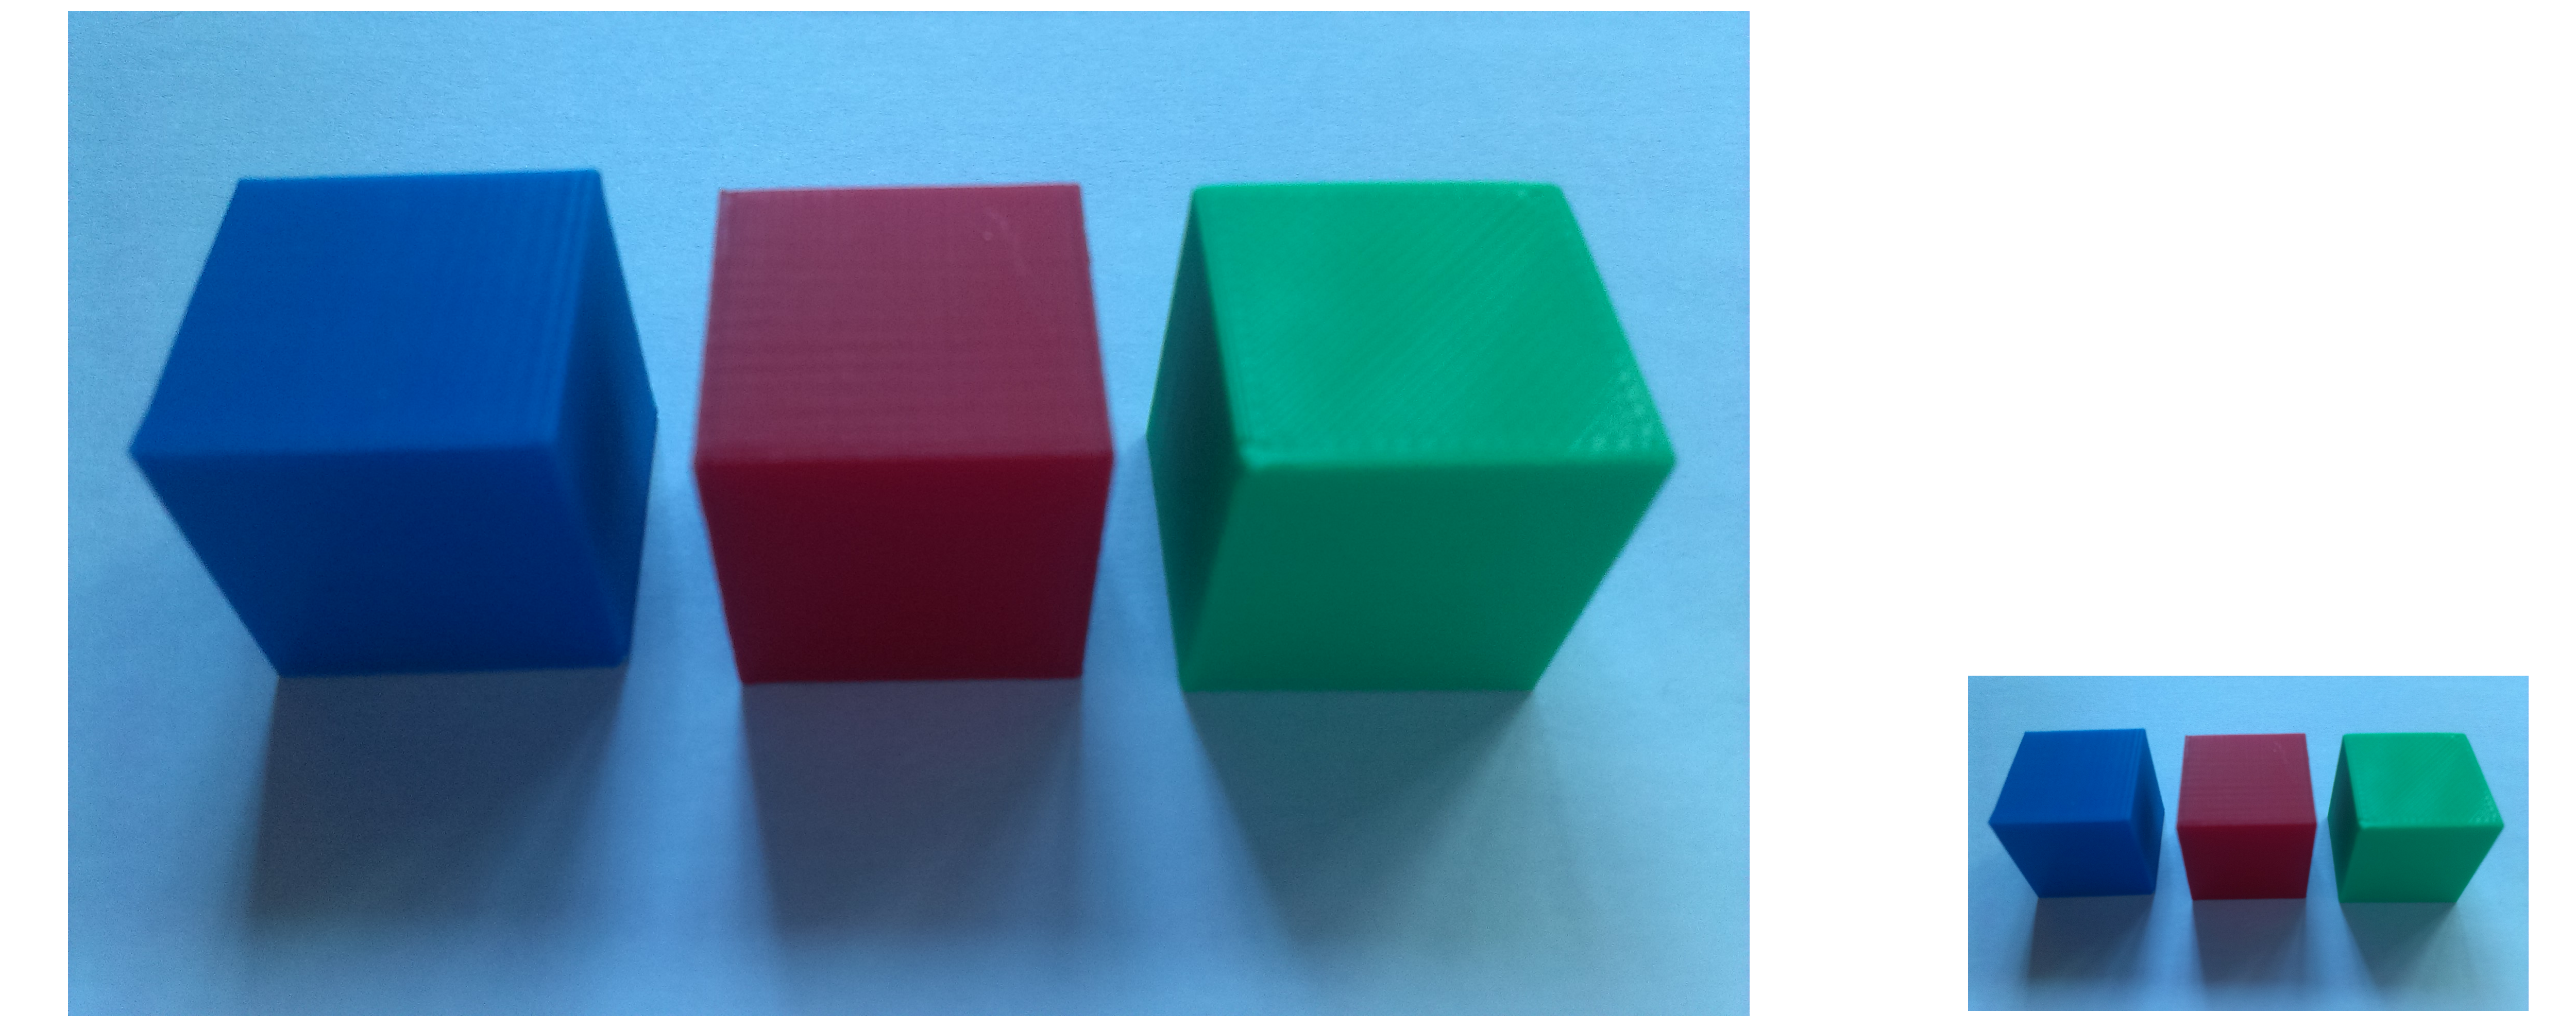
\includegraphics[width=0.6\textwidth]{img2}
  \caption{Comparación de tamaño entre imagen tomada con la cámara del teléfono y su reducción.}
\end{figure}

\noindent En definitiva, hay que tener en cuenta el tamaño que va a tener la imagen a tratar, ya que si es demasiado grande, tendremos que tener cuidado con el ruido, por lo que tendremos que aplicar técnicas de suavizado, y con imágenes demasiado pequeñas, puesto que podremos llegar a perder tanta información que el algoritmo no es capaz de reconocer nada.

\section{Segmentación}
Los primeros algoritmos de segmentación planteados fueron soluciones no demasiado buenas para la detección de los cuadrados, ya que únicamente me basaba en la característica del color de la imagen, obteniendo resultados en los que apenas se podían distinguir los cuadrados del resto del entorno.\\
Tras distintas pruebas, observé que el fondo negro era un discriminante magnífico para los colores, pero aun así, se mantenían ciertos problemas derivados del brillo.\\
Otra decisión, fue establecer el color de los cuadrados con tonalidad mate, consiguiendo mitigar el brillo de los mismos.\\
Finalmente, decidimos incluir una nueva característica, la forma de los cuadrados, para conseguir distinguirlos del fondo.\\\\
El proceso de segmentación actual es el siguiente:

\begin{enumerate}
\item Aplicamos el algoritmo de \textit{Canny} para obtener los bordes de la imagen.
\begin{figure}[h!]
  \centering
      \includegraphics[width=0.5\textwidth]{img3}
  \caption{Bordes obtenidos por el algoritmo de Canny.}
\end{figure}

\item Se aplica una clausura, es decir, ``\textit{dilato}'' el píxel y luego lo ``\textit{adelgazo}'' (lo erosiono). Con esto conseguimos terminar de cerrar los contornos de los cuadrados, consiguiendo figuras totalmente cerradas.
\begin{figure}[h!]
  \centering
      \includegraphics[width=0.9\textwidth]{img4}
  \caption{Comparación entre la imagen con los bordes y la imagen tras aplicar la clausura.}
\end{figure}

\item Dada la imagen con los bordes cerrados, localizo los contornos.
\begin{figure}[h!]
  \centering
      \includegraphics[width=0.5\textwidth]{img5}
  \caption{Contornos localizados.}
\end{figure}

\item De todos los contornos, únicamente me quedo con los que se encuentran en el nivel 2 de profundidad.
\begin{figure}[h!]
  \centering
      \includegraphics[width=0.9\textwidth]{img10}
  \caption{Contornos de nivel 2.}
\end{figure}

\item Una vez tengo los contornos de los cuadrados, ya puedo moverme por ellos pudiendo seleccionar cualquiera de los cuadrados para conocer otra característica (en este caso, el color). Para poder empezar a moverme por ellos, les extraigo el fondo aplicando una imagen binaria (conocida como máscara) obtenida tras rellenar los contornos localizados en el paso anterior.
\begin{figure}[h!]
  \centering
      \includegraphics[width=0.9\textwidth]{img11}
  \caption{Imagen original a la que le aplico la máscara, obteniendo la separación de los objetos del fondo}
\end{figure}


\end{enumerate}
Finalmente, ya tenemos extraidos los cuadrados del fondo, terminando así, la fase de segmentación.

\definecolor{shadecolor}{gray}{0.7}
\begin{shaded}
\textbf{Aclaración}. Se ha de concretar que estos elementos básicos se encuentran dentro de la secuencia, ya que al fin y al cabo deseamos que estas actividades sean ejecutadas de forma secuencial.
\end{shaded}



\end{document}
